\chapter{Introduction}
\label{CHAP::INTRODUCTION}

The scientific objective of this dissertation is a study of very high
energy ($>$350\,GeV) \Gray emission from unidentified 100\,MeV
sources.  EGRET, the Energetic Gamma-Ray Experiment Telescope, a
satellite experiment, detected \Grays from $~271$ sources at energy
$>100$\,MeV. Of these sources, 170 have yet to be identified with
objects at other wavelengths. This chapter presents a brief history of
the field of high energy (HE) and very high energy (VHE)
\Gray astronomy and introduces the EGRET experiment and its catalog of
point sources. A description of the ground-based, Whipple \Gray
detector is given and the catalog of VHE sources is summarized.

The classes of objects which have been either identified or suggested
as HE sources of \Grays are presented in
chapter~\ref{CHAP::SOURCES}. A brief review of the VHE \Gray detection
technique and of the detector system on the Whipple telescope is given
in chapter~\ref{CHAP::TECHNIQUE}. The two-dimensional reconstruction
technique, which is used to infer the origin of \Gray events and map
the VHE emission in the field of view of the telescope is described in
chapter~\ref{CHAP::ANALYSIS}. The 19 sources chosen for the survey and
the VHE sky maps of the neighborhood of these sources is presented in
chapter~\ref{CHAP::OBSERVATIONS}. A simulation study of the
characteristics of the VERITAS array, a next-generation VHE \Gray
instrument is presented in chapter~\ref{CHAP::VERITAS}. Finally, the
results of this survey are summarized and the potential for future
surveys with upcoming \Gray instruments, such as VERITAS, is discussed
in chapter~\ref{CHAP::CONCLUSIONS}.

\section{A brief history of observational gamma-ray astronomy}
\label{SEC::INTRODUCTION::HISTORY}

The field of observational high energy \Gray astronomy traces its
origins to the discovery of emission from the pulsar in the Crab
Nebula with large balloon-borne detectors in the late 1960s and early
1970s \citep[see for example][]{REF::BROWNING::NATURE1971,
REF::ALBATS::NATURE1972, REF::PARLIER::NPS1973,
REF::MCBREEN::APJ1973}. The sensitivity of balloon borne experiments
were ultimately limited by the difficulty in separating HE \Grays
originating from the relatively weak
\Gray sources from the overwhelming background of secondary charged
particles in the atmosphere. Many source detections were claimed
during this period, all with low statistical significance; only the
Crab pulsar stood the test of time.

In 1972 NASA launched the second Small Astronomy Satellite (SAS-2), a
HE \Gray satellite, comprising of a set of spark chambers which
provided energy and direction estimates for \Grays with energy
$>$35\,MeV. SAS-2 was NASA's second dedicated HE \Gray telescope, and
its fourth to carry HE \Gray detectors, after Explorer-XI
(1961), OSO-3 (1967) and OGO-5 (1968)\footnote{In addition, two
military satellites launched from the USSR contained scientific
\Gray packages which predate SAS-2: COSMOS-208 (1966) and COSMOS-264
(1969).}. These pioneering satellites had demonstrated the existence
of a flux of cosmic \Grays from the Galaxy, tentatively at first
\citep{REF::KRAUSHAAR::APJ1965}, then conclusively by mapping the
correlation of the flux with Galactic latitude and longitude
\citep{REF::CLARK::APJ1968}. They had not, however, been able to
identify any isolated \Gray sources.  This changed with the SAS-2
mission, which, in addition to measuring the diffuse Galactic \Gray
emission and finding evidence of emission from the Gould Belt (see
chapter~\ref{CHAP::SOURCES}), detected four isolated sources of
{\Grayc}s: the Crab and Vela pulsars, Cygnus X-3 and the first
unidentified high energy source, $\gamma$195$+$5
\citep{REF::FICHTEL::APJ1975, REF::HARTMAN::APJ1979}. The \Gray
excesses corresponding to these objects were large but not well
localized; the SAS instrument had an angular resolution of
$\sim2^\circ$, making identification with known sources impossible on
the basis of position alone. Association of these excesses with known
sources was done using a timing analysis, by identifying pulsations in
the \Gray signal at the known radio periods from the Crab and Vela
pulsars. In the case of Cygnus X-3, the 4.8\,hr. orbital period seen in
x-rays was used to make the identification. After six months of
operation, the satellite incurred a power supply failure and was
decommissioned.

The next advance in HE \Gray astronomy came with the launch of the
COS-B satellite, a European Space Agency mission, in 1975. COS-B was
most sensitive to \Grays in the energy range $~\sim$150\,MeV and
5\,GeV. The instrument was designed for a two year mission, but
operated for close to seven. Data from the first three years of
observations were compiled into a catalog of point sources
\citep{REF::SWANENBURG::APJ1981}, illustrated in 
figure~\ref{FIG::INTRODUCTION::2CGCATALOG}. The catalog lists 25 sources,
mostly on the Galactic plane, with four source identifications (Crab,
Vela, 3C273 and the $\rho$-Ophiuchi cloud complex), leaving 21
unidentified sources, one of which, 2CG~195$+$04, corresponds to the
unidentified SAS-2 source. Cygnus~X-3 is noticeably absent from the
COS-B catalog, the 4.8\,hr periodicity in the SAS-2 and x-ray data was
not detected; \citet{REF::MATTOX::BAAS1990} show that the periodicity
was only observed at $E<100$\,MeV by SAS-2 and would not be visible to
COS-B. The identification of 3C273 yielded the first observation of an
extra-galactic source in HE {\Grayc}s, a class of object that would be
expanded dramatically by the next generation HE \Gray instrument,
EGRET, described in detail in
section~\ref{SEC::INTRODUCTION::EGRET}. The achievements of the COS-B
mission are summarized by \citet{REF::BENNETT::NPBPS1990}.

\begin{figure}[t]
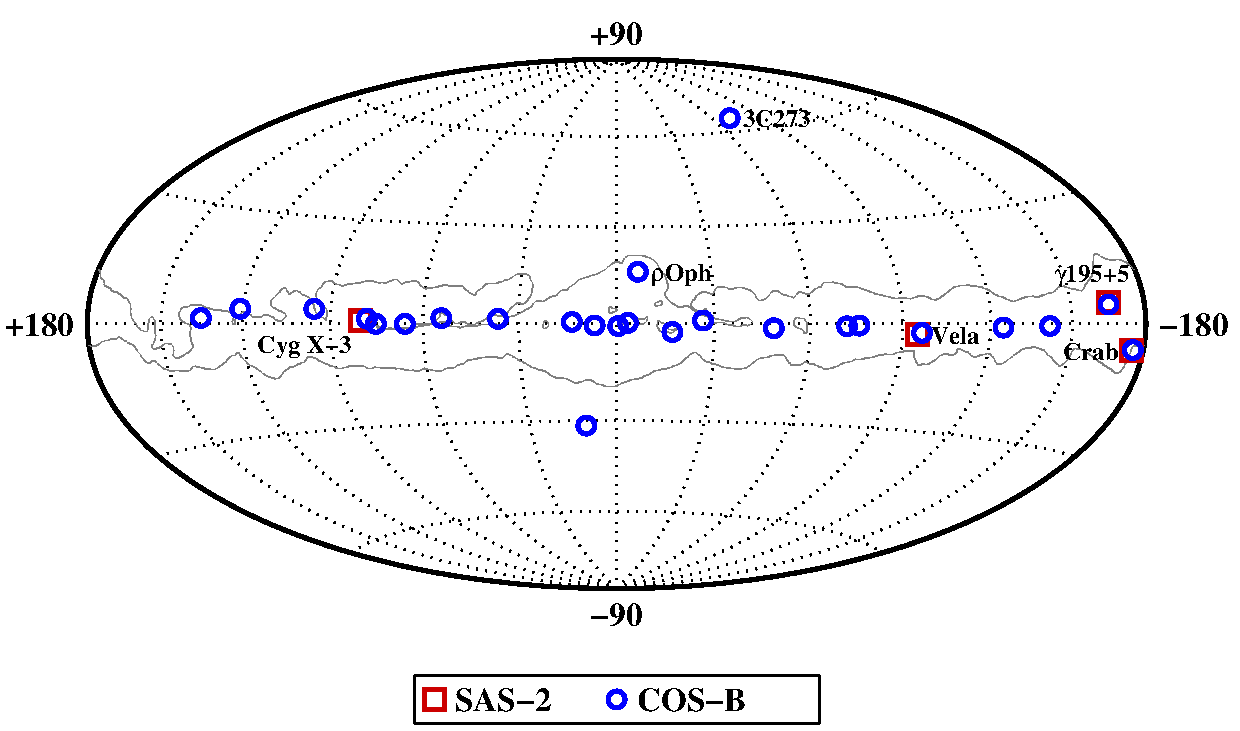
\includegraphics[angle=270,width=\textwidth]{plots/chap-introduction/2cg_catalog.pdf}
\caption{\label{FIG::INTRODUCTION::2CGCATALOG} The four identified SAS-2
sources and the 25 sources in the second COS-B catalog. Twenty one
COS-B sources were unidentified. The sources are plotted in Galactic
coordinates, with the outline of the Milky Way, from optical
observations \citep{REF::VIEIRA::2000}, displayed for comparison. The
Galactic-center is in the center of the diagram.}
\end{figure}

Contemporaneous with the development of space-based, HE \Gray
astronomy, the field of very high energy \Gray astronomy, was being
developed \citep{REF::WEEKES:BOOK2003}. In this energy regime,
instruments exploit the fact that the highest energy \Grays interact
in the atmosphere giving rise to extensive air-showers (EAS),
electromagnetic cascades of electrons, positrons and {\Grayc}s. At the
highest energies, $>10$\,TeV, arrays of scintillation detectors or
water \Cerenkov detectors placed at the high altitudes can detect
these secondaries directly and, given sufficient ground coverage, can
infer the properties of the primary from the distribution of particles
on the ground. For example, the Tibet Air-shower Array consists of
$\sim700$ detectors, distributed over an area of 36,900\,m$^2$ at an
altitude of 4,300\,m.

At lower energies, in the range of 100\,GeV -- 10\,TeV, where energy
losses to the atmosphere mean that the air shower does not have a high
charged paricle density at ground level, an indirect approach to air
shower detection is employed. \Cerenkov light emitted from the
relativistic charged secondaries can be detected at ground level by an
optical detector, usually consisting of a large mirror and array of
photo-multiplier tubes (PMTs). The diameter of the pool of light,
created by an air shower is typically greater than $200$\,m, dictated
largely by the angle of \Cerenkov light emission in the atmosphere and
by broadening of the shower through multiple Coulomb scattering of the
secondaries. \Cerenkov radiation is therefore visible at ground level
over an area of $>$10$^5$\,m$^2$, giving a huge potential effective
area to a detector that can effectively separate \Gray induced EAS
from those that result from the overwhelming background of charged
cosmic rays \citep{REF::JELLEY_PORTER::QJRAS1963}. Initial experiments
employed large ``light buckets'', such as recycled military
search-lights, to search for excesses of EAS in the direction of
potential sources \citep[see previous reference
and][]{REF::CHUDAKOV::ICRC1963}.  No statistically significant
excesses were found.

To date, two types of ground-based \Cerenkov detector have been
successful in detecting VHE \Gray emission at a statistically
significant level: instruments based on the optical \textit{imaging}
of the \Cerenkov photons with a large telescope and
\textit{non-imaging} detectors which operate in an analogous way to
air shower arrays, by using the density and temporal distribution of 
\Cerenkov light on the ground to infer the properties of the primary. 
Both techniques have a long history 
\citep{REF::WEEKES_TURVER::RAGR1977,REF::DANAHER::SOLAR1982}, and each
has resulted in the detection of point sources of {\Grayc}s. The
successful non-imaging instruments, such as STACEE and CELESTE, employ
solar furnace facilities. In these instruments, an array of large
mirrors\footnote{Usually called \textit{heliostats}, reflecting their
origins in the world of solar energy physics.} reflect light from
different parts of the \Cerenkov pool to a central station which
contains a set of PMTs. An electronic trigger system and a set of
analog-to-digital converters record the distribution and dispersion in
arrival times of photons in the light pool. On the basis of the
arrival times and intensities, \Gray events can be selected over the
background. Although this technique was initially investigated over 20
years ago, it was abandoned until more recent times, and has not yet
been exploited as fully as the imaging technique.

The imaging atmospheric \Cerenkov technique was initially suggested by
\citet{REF::WEEKES_TURVER::RAGR1977}. In essence, a large optical
telescope and high resolution camera is used to take a ``picture'', in
\Cerenkov light, of the shower development \citep{REF::FEGAN::NIM1983}. 
Although the images of \Gray induced showers are superficially similar
to those of hadronic showers, there are sufficient differences in the
development of these showers that the images can be used to
differentiate them, at least in a probabilistic sense. The images also
allow the energy and arrival direction of the primary \Grays to be
estimated, two of the basic requirements for doing astronomy at any
energy. The imaging technique was pioneered at the Fred Lawrence
Whipple Observatory in southern Arizona, leading to the first
statistically significant detection of a VHE source; the Crab Nebula
at a 9$\sigma$ confidence level \citep{REF::WEEKES::APJ1989}. Details
of the atmospheric imaging technique are given in
chapter~\ref{CHAP::TECHNIQUE}, and the Whipple 10\,m telescope is
described below. Today, ground-based instruments using the imaging
technique are operated by six groups around the world, giving coverage
in both the northern and southern hemispheres. The number of credible
VHE sources has risen to 18, including both galactic and
extra-galactic sources. A number of groups are building
next-generation ground-based detectors which will come on-line over
the next few years and which are expected to increase the number of
VHE sources significantly. Details of the design of one such
experiment, VERITAS, are given in chapter~\ref{CHAP::VERITAS}.

\section{The first unidentified HE gamma-ray source}
\label{SEC::INTRODUCTION::GEMINGA}

The case of the earliest unidentified \Gray source, which came to be
known as \textit{Geminga}\footnote{\textit{Geminga}: its name
indicates that it is a \textit{ga}mma-ray source in the constellation
\textit{Gemin}i, but see \citet{REF::BIGNAMI::APJ1983} for its
coincidental meaning in the Milanese dialect.}, is an interesting
one. A significant excess of events over the expected diffuse Galactic
emission was first seen by SAS-2 and subsequently by COS-B. The SAS-2
group reported a pulsation, with period $\sim$59\,s, in the \Grays
detected, although the limited number events (121 over four months)
and the number of degrees of freedom in the blind pulsation search
(three: phase, period and its derivative) led them to conclude that
the pulsation was not statistically compelling. At the time of
publication, four weak radio sources were known within the error box
of the data, two supernova remnants bordered it and a known satellite
galaxy to the Milky Way lay nearby. None of these associations were
convincing, and the team suggested that an undiscovered radio-pulsar
was the most likely progenitor \citep{REF::THOMPSON::APJ1977}. Despite
the investment of a significant amount of observation time, the source
remained unidentified through the COS-B era; their data did, however,
rule out the claimed $\sim$59\,s pulsation. Many claims were made
about the source during this time, but its nature remained a complete
mystery until the identification of a candidate source by the Einstein
x-ray satellite, 1E~0630$+$178 \citep{REF::BIGNAMI::APJ1983}. The
characteristics of the x-ray source were unique: large x-ray to
optical luminosity, no radio emission detected by the sensitive VLA
instrument, point-like emission in the Einstein imager and an
estimated distance of $\sim100$\,pc, placing it within the Galaxy. The
association between these objects was not conclusively made until the
ROSAT x-ray imager detected a 237\,ms pulsation
\citep{REF::HALPERN::NATURE1992} which was also seen in \Grays by the
EGRET instrument \citep{REF::BERTSCH::NATURE1992} and retrospectively in
the COS-B and SAS-2 data \citep{REF::BIGNAMI_CARAVEO::NATURE1992,
REF::MATTOX::APJ1992}. Geminga is the first example of a radio-quiet
pulsar, and serves as an illustration of the difficulty of associating
\Gray emission with objects known at other wavelengths: either
no credible object is detected in the error box of the \Gray source,
or a number are present and some characteristic of the \Gray source,
such as periodicity or variability, must be identified in one of the
prospective candidates (or vise versa as in the case of Geminga).

\section{The Energetic Gamma-Ray Experiment Telescope}
\label{SEC::INTRODUCTION::EGRET}

The Compton Gamma Ray Observatory (CGRO), launched in 1991, was the
second of NASA's ``Great Observatories''\footnote{CGRO was launched a
year after the Hubble Space Telescope and was followed by the Chandra
x-ray satellite in 1999 and recently by the SIRTF infra-red
observatory (2003).}. The observatory operated continuously until it
was de-orbited in 2000. CGRO covered the energy range from 20\,keV to
30\,GeV with its four on-board instruments: OSSE (60\,keV - 10\,MeV),
COMPTEL (800\,keV - 30\,MeV), BATSE (30\,keV - 1.9\,MeV) and EGRET
(20\,MeV to 30\,GeV). Over the course of the mission, each of the
instruments produced full sky maps of the \Gray emission within its
energy range.

\begin{figure}[t]
\resizebox{\textwidth}{!}{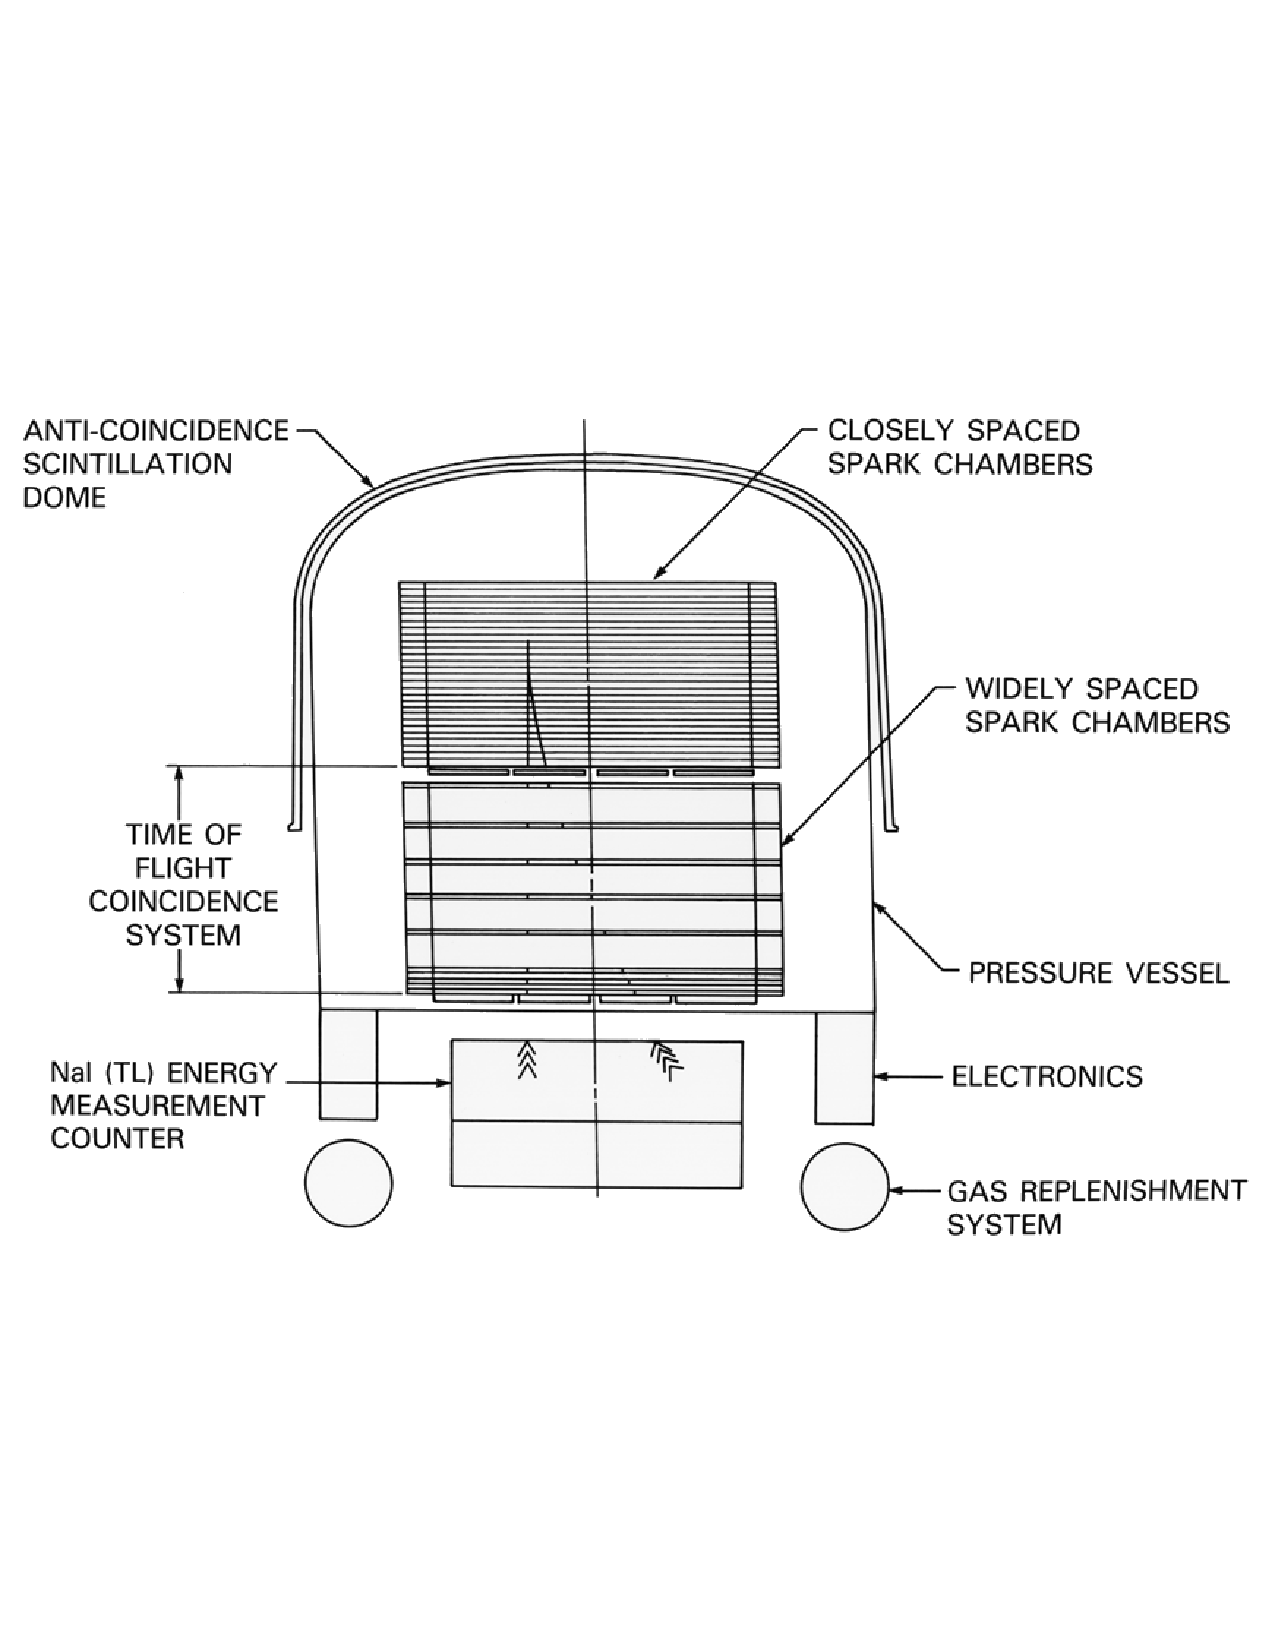
\includegraphics{plots/chap-introduction/egret-esposito.pdf}}
\caption{\label{FIG::INTRODUCTION::EGRET}Schematic of the Energetic Gamma-Ray 
Experiment Telescope (EGRET) experiment on CGRO. Two levels of spark chamber
track pair production e$^-$/e$^+$ while an NaI scintillator is used as a
calorimeter. Figure courtesy of NASA.}
%Figure reproduced from \citet{REF::THOMPSON::APJS1993}.}
\end{figure}

EGRET employed two thin-plate spark chambers to detect \Grays by
tracking electrons or positrons generated through pair-production in
the chamber. The instrument was triggered by requiring a coincident
signal to be detected in each of two sets of $4\times4$ scintillator
tiles placed under each spark chamber. The incident \Gray was required
to trigger either the corresponding tile, or neighboring tiles at each
level, to limit the angle of incidence to less than $30^\circ$. A
sodium-iodide calorimeter was used to infer the energy of the
primary. Energy resolution was $\sim$20\% up to a few GeV, above which
the particles were not fully contained in the calorimeter. Background
charged particles were eliminated by encasing the instrument in a dome
of plastic scintillator acting as an anti-coincidence shield. In
addition, upward moving particles were eliminated by measuring the
time of flight between the two scintillation layers.
Figure~\ref{FIG::INTRODUCTION::EGRET} shows a schematic of the
telescope. A detailed description of the instrument can be found in
\citet{REF::KANBACH::SSR1988}; a summary can be found in
\citet{REF::ESPOSITO::APJS1999}.

The EGRET instrument was initially planned to function for two years,
but was operated, to various degrees of efficiency, for the nine year
duration of the CGRO mission. Initially calibrated at SLAC
\citep{REF::THOMPSON::APJS1993}, the extended mission, which included
five exchanges of the spark chamber gas and numerous equipment
failures, required that the instrument be continuously recalibrated in
flight using pulsars to measure the point-spread function and the
diffuse Galactic background to check the sensitivity
\citep{REF::ESPOSITO::APJS1999}. From October 1995, EGRET was switched
from its wide field, survey mode to a narrow field, pointed mode. In
order to conserve spark chamber gas, it spent a large part of its
remaining life powered down, awaiting target of opportunity
observations of flaring AGN and \Gray bursts. EGRET's many
contributions to the field of HE \Gray astrophysics are
detailed by \citet{REF::FICHTEL::AAS1996}.

Analysis of the EGRET data for point sources was done with a maximum
likelihood method, as described by \citet{REF::MATTOX::APJ1996}. The
analysis is dependent on a complicated model of the diffuse Galactic
and extra-galactic \Gray emission which was extrapolated from radio
surveys of the Galactic gas density. The energy dependent point-spread
function and exposure, which varied by a factor of two across the sky,
was also accounted for. An iterative approach to point-source
detection was performed; a search was made for significant excesses of
\Grays above a background which included the diffuse \Gray emission
model (as described above) in addition to all those point-sources
already discovered. 

\section{Catalogs of EGRET ``point'' sources}
\label{SEC::INTRODUCTION::EGRETCATALOG}

The data produced by EGRET have been compiled into a number of catalogs
of significantly detected point sources. The EGRET team published
three catalogs of point-sources detected at energies greater than
100\,MeV, the definitive being the third EGRET Catalog
\citep{REF::HARTMAN::APJS1999}, hereafter known as the 3EG catalog.
This catalog includes data from the first four viewing periods (until
October 1995) when the instrument was in its wide-field triggering
mode. Sources are considered significant in this catalog when they are
detected above the $4\sigma$ level far from the Galactic plane, i.e.\
at Galactic latitudes of $|b|>10^\circ$. In the Galactic plane, at
$|b|<10^\circ$, a signal of at least $5\sigma$ above the background
level is required.

Source detection and localization are subject to two possible sources
of systematic error.  The model of Galactic emission is not completely
accurate; errors on small scales may lead to false detections (hence
the $5\sigma$ requirement at $|b|<10^\circ$), or more likely, lead to
systematic errors in the location of genuine sources. The iterative
approach to source identification attempts to account for the
contribution to the background of the brightest sources in the
identification of less bright ones. The large point spread function at
100\,MeV means \Grays from sources separated by distances of
$<5^\circ$ will overlap. In the analysis, this implies that sources
seperated by less than $1^\circ$ may not be resolved. Overlapping
sources can lead to systematic errors in the fitted location of each
of the sources, or to phantom sources in the catalog. Such sources
are marked as ``confused'' in the catalog. Some were later interpreted
as artifacts of very bright sources such as the Vela pulsar
\citep{REF::THOMPSON::GAMMA2001}.

\begin{figure}[t]
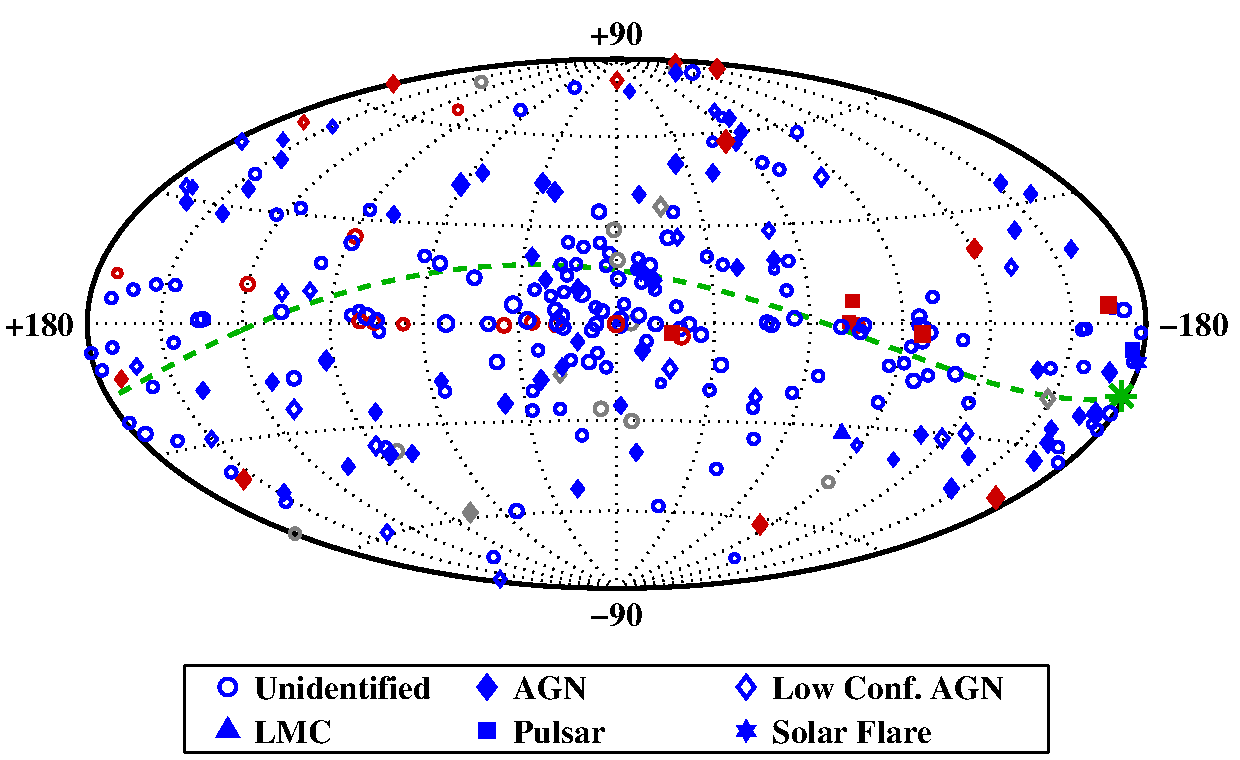
\includegraphics[angle=270,width=\textwidth]{plots/chap-introduction/3eg_catalog.pdf}
\caption{\label{FIG::INTRODUCTION::3RDEGRET} The 271 sources listed 
in the third EGRET catalog \citep{REF::HARTMAN::APJS1999}, plotted in
Galactic coordinates. Sources are displayed by source identification
(symbols) and flux (size of the symbol). Sources with a fitted
spectrum \textit{harder} than 2.0 are shown in red, those with a
softer spectrum are shown in blue. Those without an estimate of
spectral index are shown in gray. Finally, the Gould Belt is shown as
a broken green line, with the direction of the center of the Belt,
from \citet{REF::STOTHERS::AJ1974}, shown as a green star.}
\end{figure}

The catalog contains a total of 271 entries and upper limits on
emission for the remainder of the sky. For each source, maps of the
\textit{likelihood statistic}\footnote{In a likelihood analysis, the
likelihood statistic is analogous to significance. See
\citet{REF::MATTOX::APJ1996} for details.} are available, which give
the probability that the source is within a certain region of the sky at
various confidence levels.  The radius of 95\% confidence contour,
$\theta_{95}$, is quoted in the catalog as a bound on source
location. The average point source localization is
$\langle\theta_{95}\rangle=0.66^\circ$, large enough that the
error-box of many sources contains a large number of possible
counterparts at different energies, especially for those sources in
the region of the Galactic plane.

At low Galactic latitudes, 80 sources were listed in the 3EG
catalog. Five were definitively identified as known pulsars, one
corresponded to a solar flare and 74 had no unambiguous counterparts
at other energies. The 181 sources at $|b|>10^\circ$ include 66 likely
identifications with blazars, the Large Magellanic Cloud (LMC),
Centaurus A (a giant radio galaxy), 27 low confidence identifications
with AGN and 96 unidentified
sources. Figure~\ref{FIG::INTRODUCTION::3RDEGRET} shows the sources
in the 3EG catalog, by position on the sky, source type, flux
and spectral hardness.

\begin{figure}[t]
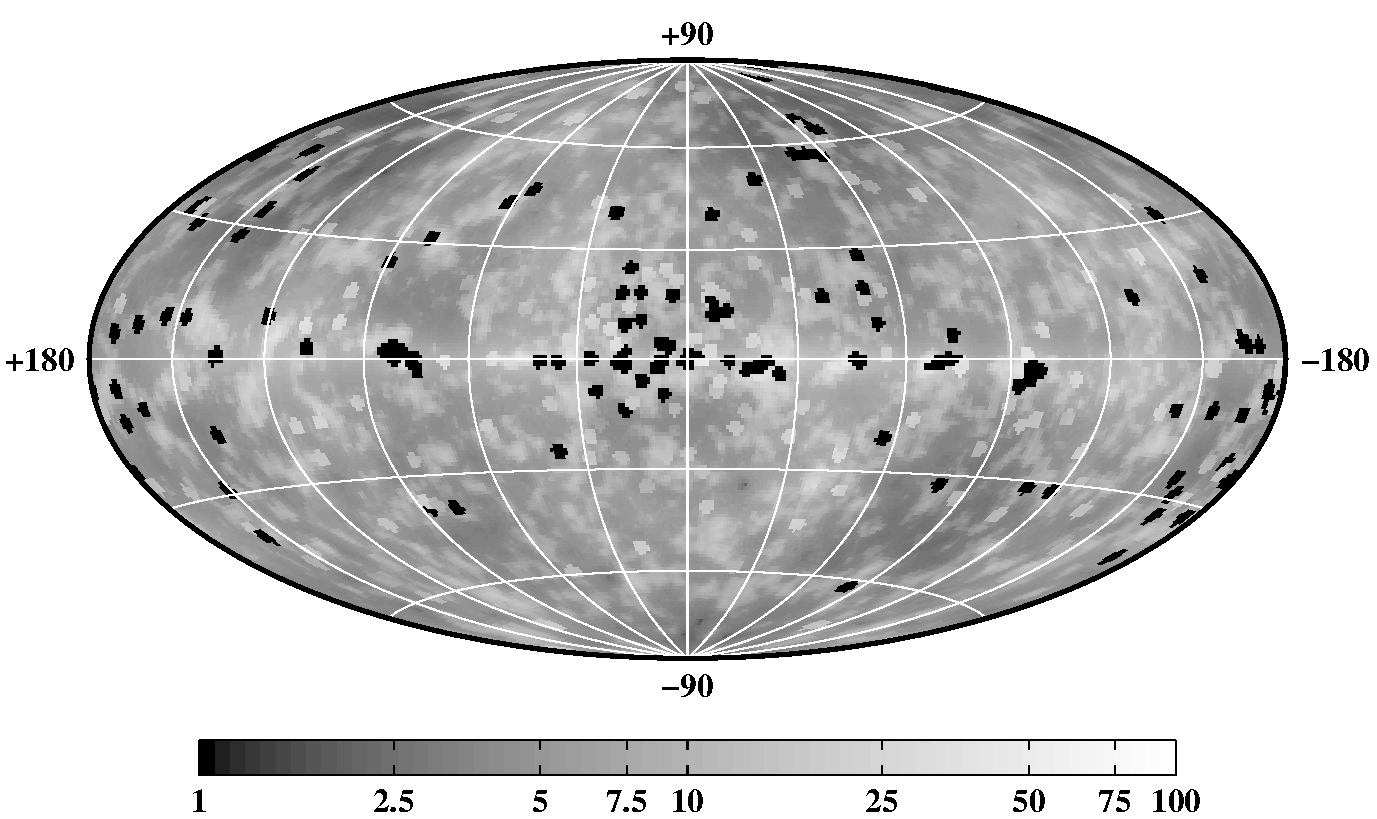
\includegraphics[draft=false,angle=270,width=\textwidth]{plots/chap-introduction/egret_ul.pdf}
\caption{\label{FIG::INTRODUCTION::3RDEGRETUL} 
Upper limits on \Gray emission at energies $>100$\,MeV from EGRET
observations, in units of $10^{-8}$\,cm$^{-2}$\,s$^{-1}$. As noted in
\citet{REF::HARTMAN::APJS1999}, the regions within $1^\circ$ of the
3EG sources are shown as black.}
\end{figure}

The majority of the detected sources are listed with flux estimates
from the viewing periods during which they were detected, and an
average flux over the full duration of the database. Many sources were
detected in each of the four viewing periods, some, such as the solar
flare, were only seen during certain portions of a single viewing
period. A systematic variability analysis of the EGRET data is
presented in \citet{REF::NOLAN::APJ2003}. Finally, the 3EG catalog
presents a power law fit to the spectrum of the detected \Grays for
those sources from which sufficiently large numbers of photons were
detected. For those parts of the sky in which no source was detected,
upper limits on emission at energies $>$100\,MeV were derived. The
limits, reproduced from the online version of the catalog, are shown
in figure~\ref{FIG::INTRODUCTION::3RDEGRETUL}. The limits represent
the maximum flux a source could have, at the 95\% confidence level,
without having been detected during the various observations by EGRET.

In addition to the third EGRET catalog, two catalogs of point-sources
detected by EGRET at higher energies have been produced. The
first, presented in two parts in \citet{REF::LAMB::APJ1997} and
\citet{REF::MACOMB::ICRC1999}, imposed a requirement that the
reconstructed energy of the \Gray be larger than 1\,GeV, and is
hereafter referred to as the GeV catalog. The production of this
catalog was motivated by the significantly smaller EGRET point spread
function at energies above 1\,GeV and by the lower background of
diffuse \Grays at these energies. It was hoped that sources could be
localized with improved accuracy and that sources with spectra harder
than the spectrum of background events would become more significant
at higher energies. A similar motivation guided the production of a
catalog of \Gray sources produced from those EGRET events with
energies greater than 10\,GeV
\citep{REF::DINGUS::GAMMA2001}, hereafter the 10\,GeV catalog. 

The first installment of the GeV catalog lists 57 sources at a
significance of $4\sigma$ and above. Ten of them had not been detected
at 100\,MeV energies in the \textit{second} EGRET catalog; a total of
thirty were listed as unidentified. The second installment of the GeV
catalog, which included data from all the EGRET viewing periods, added
another 16 sources with three that did not appear in the 3EG
catalog. The 10\,GeV catalog is based on a database of $\sim$1000
photons which were detected at large Galactic latitude; the catalog of
Galactic photons was presented at a conference but never appeared in
print. If it is assumed that the \Grays are uniformly distributed in
the sky, only two would be expected to be coincident with blazars by
chance within the EGRET point spread function. %A total of 23 photons
%were found to be coincident with AGN.

\section{Whipple 10\,m atmospheric \Cerenkov telescope}
\label{SEC::INTRODUCTION::WHIPPLE}

The Whipple 10\,m imaging atmospheric \Cerenkov telescope (IACT) is
located on Mt.~Hopkins in southern Arizona at an elevation of
2,300\,m. Built in 1968, it was the first dedicated \Gray instrument
of its type. In design, it has much in common with the large, fully
steerable, dish-type solar concentrators of the time and, indeed, it
was used as such for a brief period. For most of its life, though, it
has been operated as a ground-based \Gray telescope.  The telescope
can be operated by a single observer who chooses which sources to look
at, manages the data acquisition and analyzes the data to produce a
nearly real-time measurement of \Gray emission. The ability to produce
such a quick result has proved to be profitable on many occasions, by
prompting the telescope operator to continue to observe objects which
are in flaring states. The instrument is operated for 10 months of the
year, closing down during the summer to avoid lightning damage to the
sensitive electronics during the monsoon season.

The telescope has a total mirror area of $\sim$75\,m$^2$ and a focal
length of 7.3\,m. The mirror consists of an array of 249 identical,
spherical mirror facets, with radius of curvature 14.6\,m. The facets
are attached to a spherical optical support structure of radius
7.3\,m. This design, suggested by \citet{REF::DAVIESCOTTON::1957}, has
inferior on-axis performance when compared to a parabolic design but
has significantly improved off-axis characteristics. Since the
\Cerenkov light from an air-shower can be displaced from the direction
of the primary particle by the order of a degree or more, good
off-axis performance is important to IACT instruments. The design also
has the advantage that all mirror facets are identical and can be mass
produced. The mirrors are front aluminized at an in-house coating
facility, and anodized for protection from the environment. Front
coating improves the reflectivity in the UV band, where significant
\Cerenkov emission occurs, although it does leave the mirror coating
prone to weathering. The facets are aligned by hand at the end of each
monsoon season, and checked during the
year. Figure~\ref{FIG::INTRODUCTION::SCOPE} illustrates the design of
the telescope. As can be seen from the figure, the Davies-Cotton
design is not isochronous, a small time-spread is introduced between
parallel photons reflected from the center and edge of the mirror.

\begin{figure}[p]
\centerline{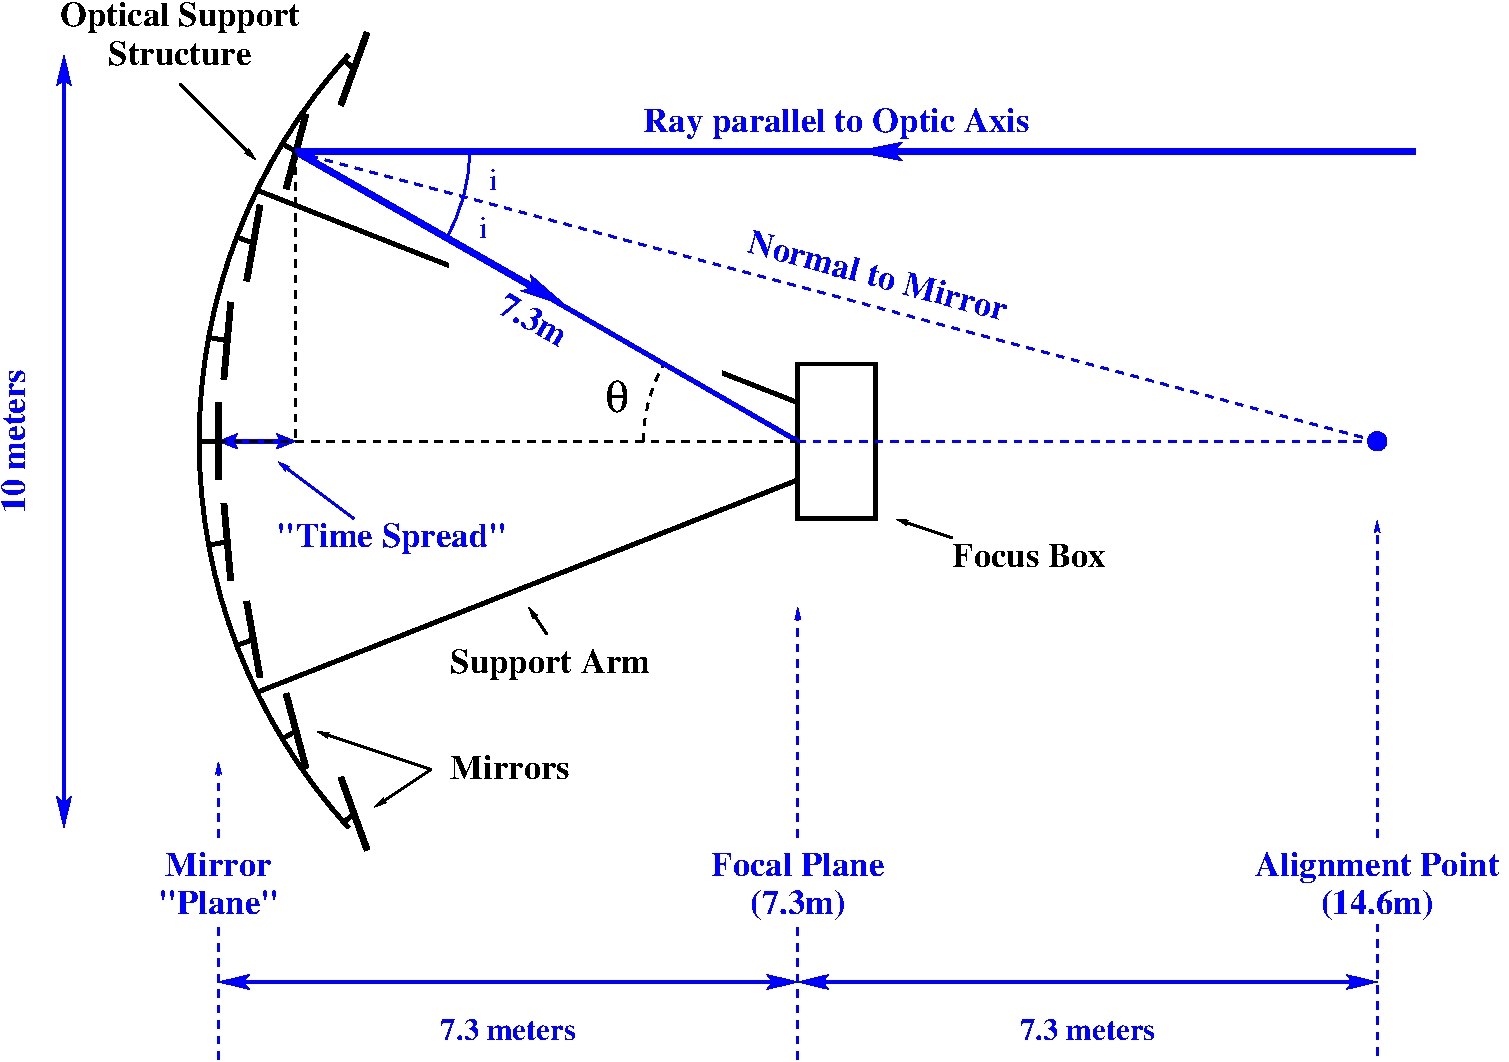
\includegraphics[height=0.4\textheight]{plots/chap-introduction/scope.pdf}}
\caption{\label{FIG::INTRODUCTION::SCOPE} Illustration of the Whipple 
10\,m telescope. The mirror consists of 249 spherical mirrors in a
Davies-Cotton configuration. The small time-spread introduced between
photons reflected from the edge and center of the mirror is evident
in the diagram.}
\end{figure}

A high resolution camera, consisting of an array of 379 1/2\,inch
phototubes in a close packed, hexagonal arrangement surrounded by 111
1\,inch phototubes, was installed on the instrument in 1999, see
figure~\ref{FIG::INTRODUCTION::PICS10M}. The PMTs have a quartz glass
window to extend their sensitivity into the UV. The voltage on each
channel is individually controllable with an Ethernet-based LeCroy
high-voltage system, allowing the gain on each channel to be equalized
across the camera. Signals from the inner 379 channels are transmitted
to the acquisition system on coaxial cables. Signals from the outer
channels are propagated on a prototype analog optical fiber system
designed to have very little dispersion. Due to the somewhat
experimental nature of the outer 111 tubes, data from them have not
been used in this survey. The inner, high resolution portion of the
camera has a field of view of $\sim2.2^\circ$.

\begin{figure}[p]
\hspace*{\fill}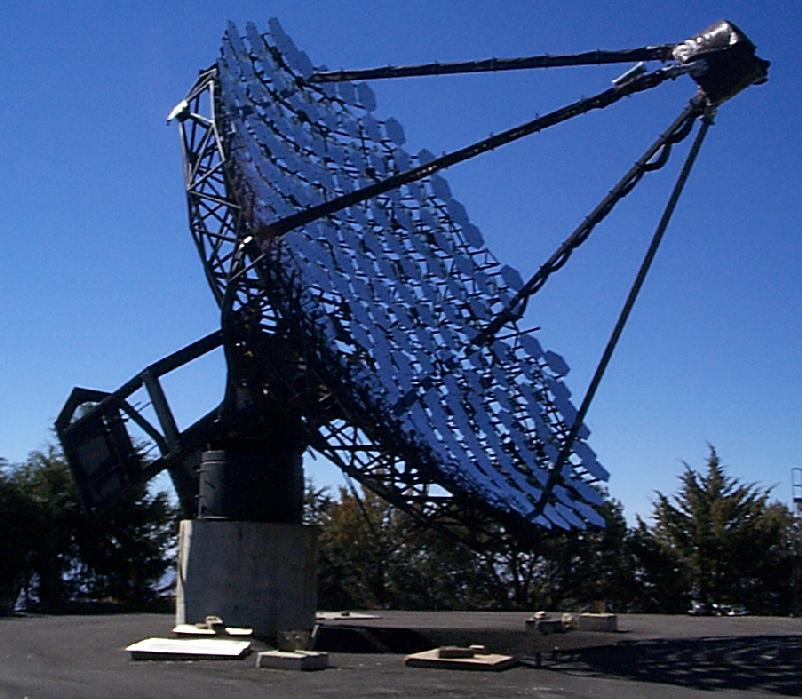
\includegraphics[height=0.25\textheight]{plots/chap-introduction/whipple99.jpg}\hspace*{\fill}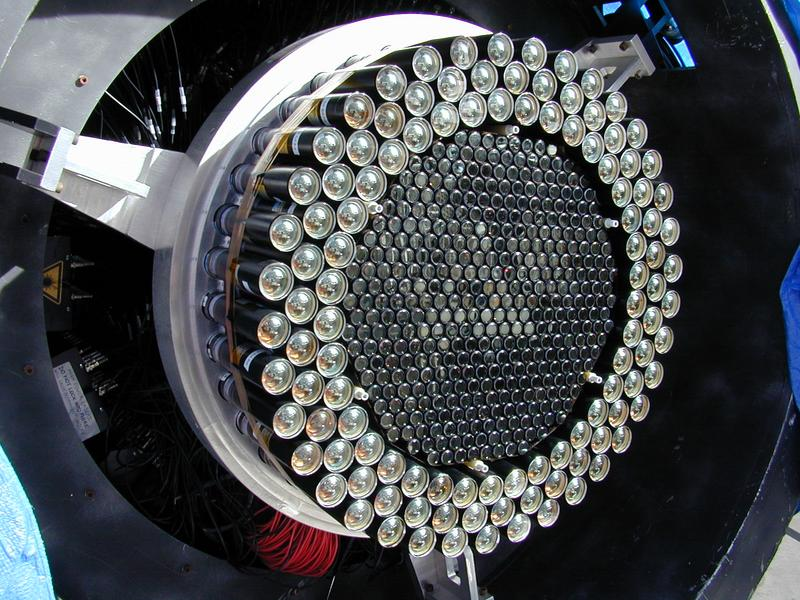
\includegraphics[height=0.25\textheight]{plots/chap-introduction/G3Camera2_small.jpg}\hspace*{\fill}
\caption{\label{FIG::INTRODUCTION::PICS10M} Left: Picture of the
Whipple 10\,m telescope (courtesy of Dr.\ R.~Lessard). Right: Picture
of the high-resolution, 499 pixel camera at the focal plane of the
instrument. In normal operation, a reflective light concentrator
plate is installed over the face of the inner 379 PMTs to increase
photon detection efficiency -- the six mounting posts for this plate
are visible between the inner and outer parts of the camera.}
\end{figure}

The instrument is triggered when three neighboring channels exceed a
preset threshold within a given coincidence time. The signals from
each channel and other information, such as the absolute time of the
event from a GPS clock and time relative to the start of the data run,
are then stored on computer for off-line analysis. Details of the
trigger electronics and data acquisition system are given in
section~\ref{SEC::TECHNIQUE::ELECTRONICS}.

The data is analyzed off-line and a set of selection criteria (called
\textit{super-cuts}) are applied to discard $>98$\% of the background
events and retain $\sim50$\% of the \Gray events. From simulations, it
is estimated that the instrument has an effective area of
$4.4\times10^4$\,m$^2$ at 1\,TeV, after data selection has been
applied. For a source with a Crab-like power law spectrum,
$dN/dE\propto(E/TeV)^{-2.5}$, the energy at which the instrument
collects most {\Grayc}s, the \textit{peak response energy} is estimated
to be $E_\mathrm{peak}$=350\,GeV. The analysis technique is described
in chapter~\ref{CHAP::ANALYSIS}.

The relatively small field of view of the ground-based \Cerenkov
instruments dictates that observations be pointed in nature. In
general, they are targeted at prospective sources for a certain number
of hours in the hope of detecting emission. This is in contrast to
satellite instruments which tend to operate in a sky survey mode, at
least for the first few years of their life. There have been some
exceptions to this rule, such as the sky-survey performed with the
Whipple telescope before the adoption of the imaging technique
\citep{REF::WEEKES::ICRC1979} and the recent survey of the Galactic plane
region with the HEGRA telescope \citep{REF::AHARONIAN::AA2002}. 

\begin{table}[p]
\caption{\label{TAB::INTRODUCTION::INSTRUMENTS}
Comparison of the characteristics of the EGRET instrument on CGRO and
the Whipple 10\,m atmospheric \Cerenkov imaging telescope.}
\centerline{\begin{tabular}{lll}\hline
Characteristic & EGRET & Whipple \\\hline
Energy Range & & \\
(MeV) & 
\raisebox{1.5ex}[0pt]{30 to $3\times10^4$} & 
\raisebox{1.5ex}[0pt]{$3\times10^5$ to $3\times10^7$} \\[1.5ex]
%Energy Resolution & 20\% & 30\% \\
%($\Delta$E/E) & 100\,MeV to 2\,GeV & 300\,GeV to 10\,TeV \\[1.5ex]
Effective Area & 1200 at 100\,MeV & $2\times10^8$ at 350\,GeV \\
(cm$^2$) & 1600 at 500\,MeV & 
$4.4\times10^8$ at 1\,TeV \\
&  1400 at 3000\,MeV &
$3.6\times10^8$ at 10\,TeV \\[1.5ex]
Average error in & 5.85 at 100\,MeV & \\ 
% Whipple - Delta(Trans) = 0.29 / 0.10   Delta(Long) = 0.26 / 0.21
% Combined -- Delta(Combined) 0.275 @ 300GeV / 0.164 @ 1TeV
% => 68% containment = 1.5 x Delta(Combined) --- 0.41667 / 0.24849
\Gray origin -- $\theta_{68}$ & 1.71 at 1\,GeV & \raisebox{1.5ex}[0pt]{0.42 at 300\,GeV} \\
(degrees) & 0.50 at 10\,GeV & \raisebox{1.5ex}[0pt]{0.25 at 1\,TeV} \\[1.5ex]
Field of view & $\sim$0.6\,sr & 0.0012\,sr \\[1.5ex]
Sensitivity to Crab& $6\times10^{-8}$ $>$ 100\,MeV & 
$3.02\times10^{-11}$ $>$ 350\,GeV\\
like spectrum & (3$\sigma$ after 2 weeks & or 0.294 $\times$ Crab flux \\
% 2001/2002 crab rate - ON 13263, OFF 8949, TIME 94128.2 sec, EXCESS 4314
% SENSITIVITY IN 5HRS IS 0.3700 crab (5 sigma) / 0.2935 crab (4 sigma)
% Integral Crab-rate from Hillas et al. is I(>350 GeV)=1.03 x 10^-6/m^2/s
(cm$^{-2}$s$^{-1}$) & off Galactic plane) & (4$\sigma$ in 5\,hrs)\\\hline
\end{tabular}}
\end{table}

Table~\ref{TAB::INTRODUCTION::INSTRUMENTS} contrasts the
characteristics of the EGRET and Whipple instruments. Whipple has
considerably better point-source localization ability than EGRET and
has a field of view comparable to the average error-box of
unidentified sources in the 3EG catalog. The Whipple instrument has a
detection sensitivity of approximately 30\% of the Crab flux in 5
hours of observation -- given a required detection at the $4\sigma$
level. Figure~\ref{FIG::INTRODUCTION::SENSITIVITY} shows the
upper limit on the luminosity of an object\footnote{At a 99\%
confidence level, used throughout this survey.}, above 350\,GeV, which
can be derived from a \textit{non-source}, through observations of
0.5, 5 and 50 hours. The hypothetical EGRET source, is chosen to have
the mean flux and spectral index (and 1$\sigma$ errors on each) of the
sources chosen for this VHE survey.

\begin{figure}[p]
\centerline{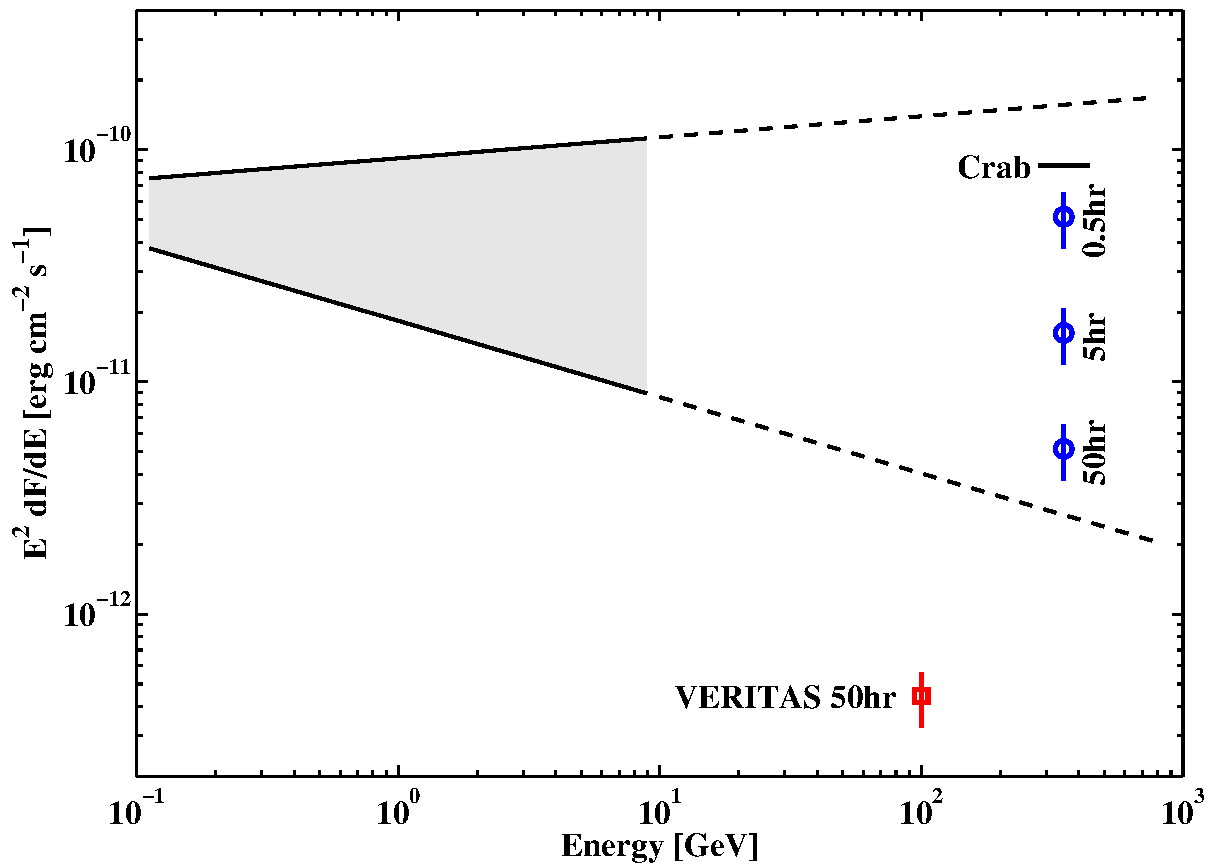
\includegraphics[angle=270,width=0.75\textwidth]{plots/chap-introduction/sensitivity_VHE_3eg_VERITAS.pdf}}
\caption{\label{FIG::INTRODUCTION::SENSITIVITY} 
Comparison of upper limit on source luminosity derivable through
observations at Whipple with the extrapolated luminosity of a ``mean''
100\,MeV source. Upper limits for 0.5, 5 and 50 hour observations are
shown, assuming a Crab-like spectrum. The hypothetical 100\,MeV
source, has an integral flux spectrum given by the mean flux and
spectral index from 3EG sources chosen for this survey:
$I(>E)=(30.9\pm4.1)\times10^{-8}(E/100MeV)^{-1.12\pm0.21}$\,cm$^{-2}$s$^{-1}$.}
\end{figure}

\section{Catalog of VHE gamma-ray sources}
\label{SEC::INTRODUCTION::VHECATALOG}

To date, 18 credible source detections have been made by ground-based
\Gray community. These sources are listed in
table~\ref{TAB::INTRODUCTION::VHESOURCES} and are plotted in
figure~\ref{FIG::INTRODUCTION::VHECATALOG}. Nine have been confirmed
by more than one ground-based instrument and are considered to be
beyond dispute. The others are, as yet, unconfirmed. In some of these
cases the discoveries are so recent that sufficient observations have
not been made by an independent group. In others cases it is because
there is no longer an independent telescope operating in the correct
range of latitude to provide confirmation. In the case of 3C66A, a
blazar discovered in 1998, it is possible that the initial discovery
was made during a period of extreme flaring activity, which has not
been repeated. In the case of Cen~X-3, flaring outbursts have been
noted at other wavelengths, but the VHE emission was reported to be
steady over the course of the observation. Since they are expected to
be persistent, and have not been confirmed, the discoveries of Vela
and Cen~X-3 have therefore been regarded as grade ``\textit{C}''
\citep{REF::HORAN_WEEKES::2NDVERITAS2004}.

\begin{table}[t] 
\caption{\label{TAB::INTRODUCTION::VHESOURCES}Catalog of published VHE 
sources$^1$. Adapted from \citet{REF::HORAN_WEEKES::2NDVERITAS2004}.}
\begin{centering}
\begin{tabular}{lllllll}\hline
Src.     & VHE catalog & Associated   & Source   & Discovery & 3EG     & Indep. \\
no.$^2$  & name      & source         & type & year/group$^3$& src.    & conf.  \\\hline
1  & TeV~0047$-$2518 & NGC 253        & Starburst  & 2003/C  & No      & No  \\
2  & TeV~0219$+$4248 & 3C66A          & Blazar     & 1998/Cr & Yes     & No  \\
3  & TeV~0535$+$2200 & Crab           & SNR/PWN    & 1989/W  & Yes     & Yes \\
4  & TeV~0834$-$4500 & Vela           & SNR/PWN    & 1997/C  & No      & No  \\
5  & TeV~1121$-$6037 & Cen X$-$3      & Binary     & 1998/D  & Yes     & No  \\
6  & TeV~1104$+$3813 & Mrk 421        & Blazar     & 1992/W  & Yes     & Yes \\
7  & TeV~1231$+$1224 & M87            & Radio Gal. & 2003/H  & No      & No  \\
8  & TeV~1429$+$4240 & H1426$+$428    & Blazar     & 2002/W  & No      & Yes \\
9  & TeV~1503$-$4157 & SN1006         & SNR        & 1997/C  & No      & Yes \\
10 & TeV~1654$+$3946 & Mrk 501        & Blazar     & 1995/W  & No      & Yes \\
11 & TeV~1710$-$4429 & PSR 1706$-$44  & SNR/PWN    & 1995/C  & No      & Yes \\
12 & TeV~1712$-$3932 & RXJ1713$-$3946 & SNR        & 1999/C  & No      & No  \\
13 & TeV~2000$+$6509 & 1ES1959$+$650  & Blazar     & 1999/TA & No      & Yes \\
14 & TeV~2032$+$4131 & \textit{unidentified} 
                       & \textit{unidentified}$^4$ & 2002/H  & Yes$^5$ & No  \\
15 & TeV~2159$-$3014 & PKS2155$-$304  & Blazar     & 1999/D  & Yes     & Yes \\
16 & TeV~2203$+$4217 & BL Lacertae    & Blazar     & 2001/Cr & Yes     & No  \\
17 & TeV~2323$+$5849 & Cas A          & SNR        & 1999/H  & No      & No  \\
18 & TeV~2347$+$5142 & 1ES2344$+$514  & Blazar     & 1997/W  & No      & Yes \\\hline
\end{tabular}

\footnotesize
\begin{tabular}{lp{0.95\textwidth}}
$^1$ & All VHE sources published in refereed journals are presented
here. Recent results from conferences, awaiting publication, are not
shown.\\ $^2$ & Source number from VHE source map,
figure~\ref{FIG::INTRODUCTION::VHECATALOG}.\\ $^3$ & C:~CANGAROO,
Cr:~Crimea, D:~Durham, H:~HEGRA, TA:~Telescope Array and W:~Whipple.\\
$^4$ & \citet{REF::BUTT::APJ2003} suggest that TeV~2032$+$4131 is
associated with an OB association, Cyg~OB2. Other associations have
also been made \citep{REF::MUKHERJEE::APJ2003}. \\
$^5$ & VHE source is coincident with 3EG~J2033$+$4118.
\end{tabular}
\end{centering}
\end{table}

\begin{figure}[t]
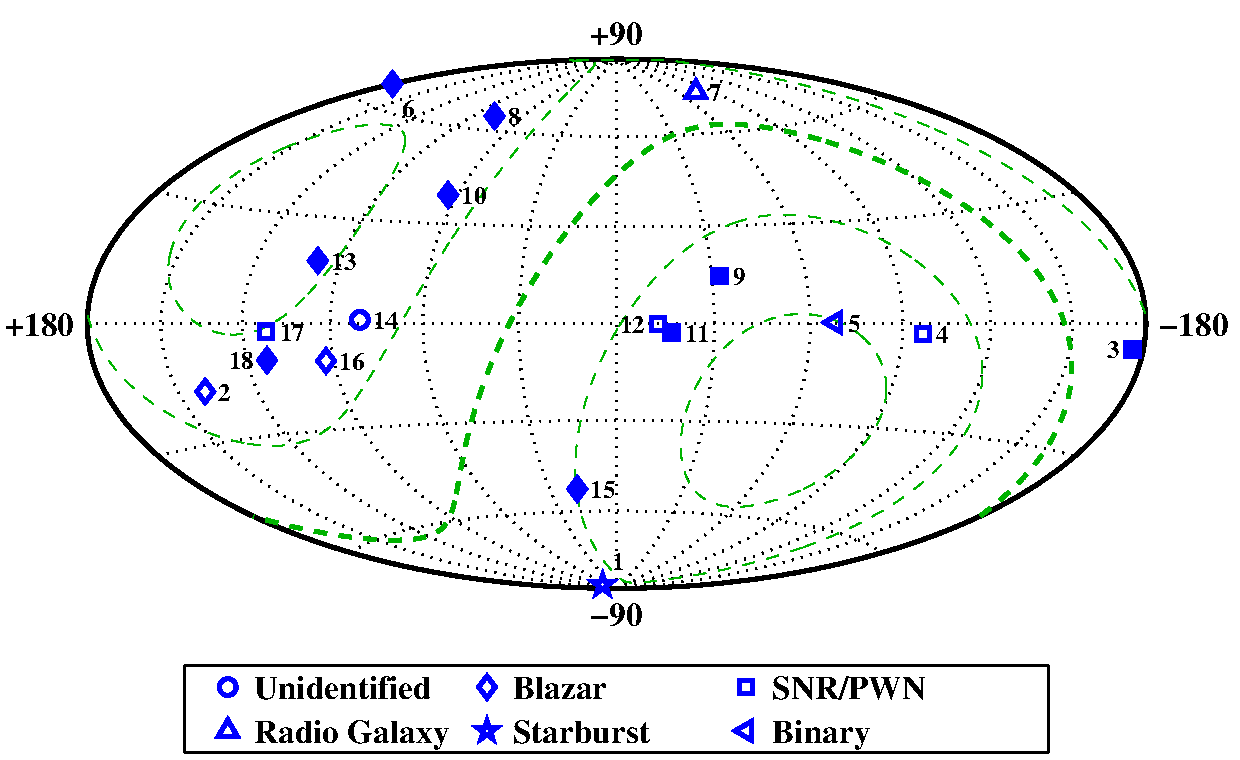
\includegraphics[angle=270,width=\textwidth]{plots/chap-introduction/tev_catalog.pdf}
\caption{\label{FIG::INTRODUCTION::VHECATALOG} 
The 18 objects reported as \Gray sources in the VHE regime, in
Galactic coordinates. Confirmed sources are depicted as solid symbols,
unconfirmed sources as outlines. Sources are listed by number, as they
appear in the VHE catalog, table~\ref{TAB::INTRODUCTION::VHESOURCES}. The
thick broken line shows the equatorial plane, separating the northern
and southern hemispheres. The thinner broken lines show the 30$^\circ$
and 60$^\circ$ declinations north and south. The data for this figure
are taken from \citet{REF::HORAN_WEEKES::2NDVERITAS2004}.}
\end{figure}

The mechanisms responsible for HE and VHE emission are discussed in
chapter~\ref{CHAP::SOURCES}. A brief list of the observational
characteristics of the sources and source types are presented below
without reference to the emission mechanisms.  

The first source detected by a ground-based \Gray instrument was the
Crab Nebula \citep{REF::WEEKES::APJ1989}. The Crab, a class of
supernova remnant (SNR) called pulsar wind nebula (or plerion -- see
section~\ref{SEC::SOURCES::PWN}), was the result of a historical
supernova explosion in the year 1054. It is a unique object, one of
the brightest in the sky over all wavelengths, with non-thermal
emission at radio, optical, x-ray and \Gray energies. Pulsations from
a central pulsar are seen at most energies up to and including the HE
\Gray range. The VHE emission from this object is consistent with
being steady over the 15 years for which it has been detected. It has
become the ``standard candle'' in the VHE regime, a source to
calibrate new instruments against. Its spectrum is well fitted by a
power-law with spectral index of $-2.49$ \citep{REF::HILLAS::1998}. No
periodicity has been seen in the VHE \Gray signal, which is not
thought to have come directly from the pulsar, but to emanate from a
synchrotron nebula surrounding it. In addition to the Crab, VHE
emission has been reported from two other pulsar wind nebulae, both in
the southern hemisphere: PSR~1706$-$44 and Vela.

The remaining SNR belong to the class of shell-type supernova
remnant. Two, SN1006 and RXJ1713$-$3946, are in the southern
hemisphere; the third, Cas~A, is in the northern hemisphere.  As
discussed in section~\ref{SEC::SOURCES::SNR}, SNR may be associated
with the acceleration of charged particles through diffusive shock
acceleration. The shape of the spectra of VHE \Grays from these
objects, in conjunction with observations at other wavelengths, is
expected to determine whether hadronic acceleration is occurring at
these sites, or whether the emission is the result of electron
acceleration. Emission from SN1006 is consistent with a purely
leptonic model, while RXJ1713$-$3946 and Cas~A may show evidence for
hadronic acceleration, see section~\ref{SEC::SOURCES::SNR}.

The VHE blazars, extra-galactic objects associated with compact
super-massive black holes (see section \ref{SEC::SOURCES::BLAZARS}),
are characterized by extreme variability on the time scales of hours
and days \citep{REF::GAIDOS::NATURE1996}. Their emission can go from a
quiescent state that is at or below the sensitivity of the Whipple
instrument to a flaring state with emission at a level of a few times
the Crab flux over the course of a single night of
observations. During these flaring periods, the spectral index of the
source has also been seen to change; in the case of Mrk~421, a
hardening of the spectrum from $-2.7$ to $-1.9$ was observed in
data from the Whipple telescope, taken during 2000/2001
\citep{REF::KRENNRICH::APJ2002}. Flaring activity at TeV energies 
is usually correlated with increased activity at other wavelengths, in
particular significant correlations with x-ray flares have been
observed \citep{REF::MARASCHI::AP1999}.

\section{VHE observations of third EGRET catalog sources}
\label{SEC::INTRODUCTION::VHE3EG}

The 170 unidentified sources in the 3EG catalog have motivated
multiwavelength studies at all wavelengths. Studies using the ASCA
x-ray satellite have revealed possible counterparts for some of them
\citep{REF::ROBERTS::APJS2001}, as have studies in the radio and
optical bands. In some cases, the multiwavelength approach has been
able to narrow the potential candidate associations, leaving a single
likely candidate. It is in the spirit of this tradition, that a survey
of unidentified sources has been undertaken with the Whipple VHE \Gray
telescope. The unidentified sources provide a catalog of objects whose
error-box is well matched to the field of view of an IACT. If VHE
emission is present, observations with an IACT would have sufficient
angular resolution to narrow down the potential candidates within the
error box of the 3EG source and, potentially, provide an unambiguous
association. This has been the scientific objective of the research
reported in this dissertation.

Objects have been chosen for the survey based upon a number of
factors. Preference was given to persistent objects, with hard spectra
for which a lack of VHE emission would necessitate a cut-off in the
spectrum. In all cases, the location of the source in the sky
influenced the choice. It is desirable that sources lie between
declinations of $10^\circ$ south and $70^\circ$ north so that they are
can be observed with the Whipple telescope at relatively small angles
from the zenith, for which the density of \Cerenkov photons on the
ground is highest. Additionally, since the telescope is operated by a
relatively large collaboration, with diverse research interests,
sources were chosen so as not to clash with areas of the sky for which
considerable conflicting interests exist, such as the Galactic Center
region. Finally, \citet{REF::PETRY::NUGH2001} extrapolated the known
EGRET spectrum of the unidentified sources to provide a table of most
likely detections with next-generation \Cerenkov instruments. A number
of the most likely sources from this list were
chosen. Chapter~\ref{CHAP::OBSERVATIONS} lists the 3EG sources chosen
in this survey and presents the results of the VHE survey.
